\newpage
\phantomsection
{\bfseries МРНТИ 30.19.29}
\hfill {\bfseries \href{https://doi.org/10.58805/kazutb.v.2.23-337}{https://doi.org/10.58805/kazutb.v.2.23-337}}

\sectionwithauthors{М.Р.Нургужин, Г.Т.Даненова, А.М.Нургужина, Т.Б. Ахметжанов}{РАСЧЕТНЫЕ ЗАВИСИМОСТИ ДЛЯ ОПРЕДЕЛЕНИЯ ЭНЕРГЕТИЧЕСКОГО J-ИНТЕГРАЛА}

\begin{center}
{\bfseries \textsuperscript{1}М.Р.Нургужин, \textsuperscript{2}Г.Т.Даненова\envelope, \textsuperscript{3}А.М.Нургужина, \textsuperscript{2}Т.Б. Ахметжанов}

\textsuperscript{1} АО «Национальный центр космических исследований и
технологий»,

Алматы, Казахстан,\textsuperscript{2} Карагандинский технический
университет имени Абылкаса Сагинова, Караганда, Казахстан,

\textsuperscript{3} Astana IT университет, г. Астана, Казахстан,

\envelope Корреспондент-автор: guldan72@mail.ru
\end{center}

Известно, что трещиноподобные дефекты существуют в изделии изначально,
требует создания методов анализа, позволяющих исследовать
распространение трещин в условиях реального нагружения на основе
механики разрушения. Широко используемыми критериями для этих случаев
являются коэффициент интенсивности напряжений, J-интеграл и критерий
раскрытия трещины. В данной статье рассмотрены численные исследования
определения \emph{J}-интеграла методом конечных элементов для
стандартных образцов, моделирующих поведение типовых сварных соединений.
В качестве таких образцов рассмотрены образцы с краевой и центральной
трещинами. С позиций регрессионного и корреляционного анализов на основе
планирования машинных экспериментов получены выражения для J-интеграла в
типовых сварных соединениях в зависимости от геометрии трещин, внешней
нагрузки и параметров материала. Решен ряд методических примеров по
определению разрушающих напряжений. Определены границы применяемости
линейной механики разрушения для краевых и центральных трещин в типичных
образцах. Оценено влияние остаточных напряжений на величину
\emph{J}-интеграла в типовых образцах. Таким образом, регрессионные
зависимости для определения \emph{J}-интеграла обладают достаточной
надежностью и могут использоваться в практике прогнозирования
остаточного ресурса сварных металлоконструкций.

{\bfseries Ключевые слова:} механика разрушения, \emph{J}-интеграл, сварные
конструкции, остаточные напряжения, распространение трещины

\begin{center}
{\large\bfseries ЭНЕРГЕТИКАЛЫҚ J-ИНТЕГРАЛЫН АНЫҚТАУҒА АРНАЛҒАН ЕСЕПТІК ТӘУЕЛДІЛІКТЕР}

{\bfseries \textsuperscript{1}М.Р. Нұрғожин,
\textsuperscript{2}Г.Т.Даненова\envelope,
\textsuperscript{3}А.М. Нұрғожина, \textsuperscript{2}Т.Б. Ахметжанов}

\textsuperscript{1}«Ұлттық ғарыштық зерттеулер мен технологиялар
орталығы» АҚ, Алматы қ., Қазақстан,

\textsuperscript{2} Әбілқас Сағынов атындағы Қарағанды техникалық
университеті, Қарағанды қ., Қазақстан,

\textsuperscript{3} Astana IT университеті, Астана қ., Қазақстан,

е-mail: guldan72@mail.ru
\end{center}

Өнімде жарық тәрізді ақаулар бастапқыдан бар екендігі белгілі, сыну
механикасы негізінде нақты жүктеме жағдайында жарықтардың таралуын
зерттеуге мүмкіндік беретін талдау әдістерін жасауды қажет етеді. Бұл
жағдайлар үшін кеңінен қолданылатын өлшемдер-кернеу қарқындылығы
коэффициенті, J-интегралы және жарықшақты ашу критерийі. Бұл мақалада
стандартты дәнекерленген қосылыстардың әрекетін модельдейтін стандартты
үлгілер үшін ақырлы элементтер әдісімен J-интегралын анықтауға арналған
сандық зерттеулер қарастырылған. Мұндай үлгілер ретінде шеткі және
Орталық жарықтары бар үлгілер қарастырылады. Машиналық эксперименттерді
жоспарлау негізінде регрессиялық және корреляциялық талдаулар тұрғысынан
жарықтардың геометриясына, сыртқы жүктеме мен материал параметрлеріне
байланысты типтік дәнекерленген қосылыстардағы J-интегралына өрнектер
алынды. Деструктивті кернеулерді анықтау бойынша бірқатар әдістемелік
мысалдар шешілді. Типтік үлгілердегі шеткі және орталық жарықтар үшін
сызықтық сыну механикасын қолдану шекаралары анықталған. Қалдық
кернеулердің типтік үлгілердегі J-интегралының мәніне әсері бағаланды.
Осылайша, J-интегралын анықтауға арналған регрессиялық тәуелділіктер
жеткілікті сенімділікке ие және дәнекерленген металл конструкцияларының
қалдық ресурстарын болжау тәжірибесінде қолданыла алады.

{\bfseries Түйін сөздер:} сыну механикасы, J интегралы, дәнекерленген
құрылымдар, қалдық кернеулер, жарықтың таралуы

\begin{center}
{\large\bfseries CALCULATION DEPENDENCIES FOR DETERMINATION OF THE ENERGY J-INTEGRAL}

{\bfseries \textsuperscript{1}M.R. Nurguzhin, \textsuperscript{2}G.T.
Danenova\envelope , \textsuperscript{3}А.M. Nurguzhinа,
\textsuperscript{2}T.B. Akhmetzhanov}

\textsuperscript{1} Joint Stock Company ``National Center of Space
Researches and Technologies'', Almaty, Kazakhstan,

\textsuperscript{2} Karaganda Technical University named by Abylkas
Saginov, Karaganda, Kazakhstan,

\textsuperscript{3} Astana IT University, Astana, Kazakhstan,

е-mail: guldan72@mail.ru
\end{center}

It is known that crack defects exist in the machines initially. All that
requires the creation of analysis methods that allow to research the
propagation of cracks under real loading conditions based on the
mechanics of destruction. Widely used criteria for these cases are
stress intensity factor, J-integral and crack opening criterion. This
paper discusses numerical research of the J-integral determination by
finite element method for typical samples that simulating behavior of
welded joints. Samples with edge and center cracks are considered as
such samples. The expressions for the J-integral in typical welded
joints are obtained from the positions of regression and correlation
analyses, based on the planning of machine experiments. These
expressions are depending on the geometry of cracks, external load and
material parameters. A number of methodological examples for determining
destructive stresses have been solved. Limits of application of linear
fracture mechanics for typical samples with edge and center cracks are
determined. Influence of residual stresses on value of J-integral in
typical samples is estimated. Thus, regression dependencies for
determining the J-integral have sufficient reliability and can be used
in the practice of predicting the residual life of welded steel
structures.

{\bfseries Keywords:} fracture mechanics, J-integral, welded structures,
residual stresses, crack propagation.

\begin{multicols}{2}
{\bfseries Введение.} Анализ разрушения сварных металлоконструкций, условий
их производства и эксплуатации на основе обследования более 400
технологических машин показывает наличие большого числа усталостных и
хрупких разрушений. Очагами разрушения сварных соединений, как правило,
являются дефекты сварки, конструктивные несплошности,
конструктивно-технологическая концентрация напряжений и деформаций
{[}1,2{]}.

Металлоконструкции технологических машин проектировались, по существу,
по принципу безопасного ресурса, в соответствии с которым в конструкции
практически не допускалось возникновение трещин за период проектного
(назначенного) ресурса. Осознание того, что трещиноподобные дефекты
существуют в изделии изначально, требует создания методов анализа,
позволяющих исследовать распространение трещин в условиях реального
нагружения на основе механики разрушения {[}2,3,4{]}. Особую роль в этом
случае для обеспечения безопасности технических объектов играет
живучесть конструкций, т.е. способность выполнять свои функции при
разрушении отдельных элементов. При этом не считается, что появление
трещин является концом работы элемента или узла конструкции.

В настоящее время поддержание эксплуатационной надежности сварных
конструкций за пределами нормативных сроков службы обеспечивается, как
было сказано выше, в рамках концепции «безопасного повреждения» системой
технических обслуживаний на основе руководящих документов.

В практике проектирования специалистами применяются апробированные
критериальные параметры, хотя они и являются частными и используют те
или иные дополнительные предположения о зоне и характере предразрушения
в вершине трещины. Широко используемыми критериями для этих случаев
являются коэффициент интенсивности напряжений, \emph{J}-интеграл и
критерий раскрытия трещины {[}3,4,5{]}.

В данной статье рассмотрены численные исследования определения
\emph{J}-интеграла методом конечных элементов (МКЭ) для стандартных
образцов, моделирующих поведение типовых сварных соединений. В качестве
таких образцов рассмотрены образцы с краевой и центральной трещинами.

{\bfseries Материалы и методы.} В развитии механики разрушения и, в
частности, в исследованиях динамического распространения трещины
концепция упругого коэффициента интенсивности напряжений сыграла
фундаментальную роль. Этот параметр линейной механики разрушения
применяется не только для анализа причин разрушения уже разрушившихся
конструкций или поиска способов предотвращения разрушения, но и с
успехом - для выявления корреляции между напряженно-деформированным
состоянием окрестности вершины трещины и скоростью распространения
усталостной трещины, а также при исследовании коррозийного
растрескивания {[}2,5{]}.

Дальнейшим развитием линейной механики разрушения явилось ее применение
в исследованиях таких процессов упругопластического разрушения, при
которых влиянием перераспределения напряжений и деформаций в зонах
упругости и пластичности нельзя пренебречь. Особенно это актуально для
материалов с умеренными прочностными характеристиками (низколегированные
и углеродистые стали, применяемые для производства большинства сварных
машиностроительных конструкций). Широко используемыми критериями для
этих случаев являются \emph{J}-интеграл и критерий раскрытия трещины
\emph{COD}. Однако известно, что \emph{J}-интеграл является параметром,
который вводится при некоторых ограничительных условиях; что же касается
\emph{COD}, то измерить точно на практике его не удается. Применение
критериев механики разрушения для анализа прочности сварных конструкций
усложняется в связи с их спецификой, связанной с наличием остаточных
напряжений и деформаций, конструктивно-технологической концентрацией
напряжений в зонах сварных соединений и т. п. {[}1,2,4{]}.

Рассмотрим энергетический J-интеграл и его вычисление на основе метода
конечных элементов. При оценке прочности сварных соединений важно иметь
упрощенные выражения для оперативной оценки параметров механики
разрушения. С позиций регрессионного и корреляционного анализов на
основе планирования машинных экспериментов получены выражения для
определения J-интеграла в типовых сварных соединениях в зависимости от
геометрии трещин, внешней нагрузки и параметров материала.

Учитывая симметрию, для 1/2 части образца с одной краевой трещиной
построена дискретная модель (рисунок 1).
\end{multicols}

\begin{figure}[H]
	\centering
	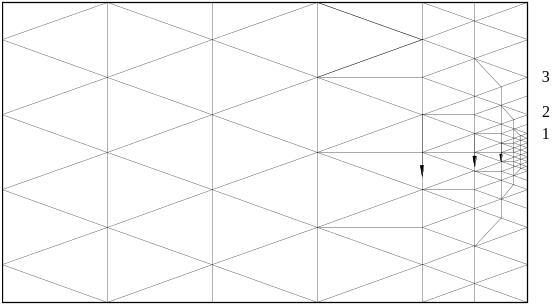
\includegraphics[width=0.8\textwidth]{assets/1134}
	\caption*{Рис. 1 - Дискретная модель для 1/2 части образца с одной краевой трещиной}
\end{figure}

\begin{multicols}{2}
Следует обратить внимание на контуры интегрирования, которые обозначены
на этом рисунке 2. Задача решалась по двум расчетным схемам: плоская
деформация (ПД) и плоское напряженное состояние (ПНС), на основе теории
течения. В качестве материала рассмотрена сталь с параметрами:
$E = 2.1 \cdot 10^{5} \text{МПа;}$ $\sigma_{T} = 490 \text{МПа};$ $\nu = 0.3;$ $E_{T} = 2100 \text{МПа}.$

Сравнение значений $J$ - интеграла при
решении упругопластической и упругой задач показано на рисунке 2 и 3. В
работе {[}9{]} показано, что линейная механика разрушения может
применяться вплоть до нетто-напряжения
$\sigma_{H} = 0.8 \sigma_{T}$ для краевых трещин в массивных телах
глубиной менее 0,25 сечения или для поверхностных трещин размером менее
половины сечения. Анализ полученных результатов показал, что пределы
применимости линейного подхода сильно зависят от степени стеснения
деформации, размеров дефектов и уровня напряжения в нетто-сечении. Так
для краевой трещины в случае плоского напряженного состояния с ошибкой в
15\% для трещин $\frac{l}{b} = \frac{0.1}{0.5}$ величина границы
применимости линейной механики разрушения изменяется в пределах
$\left( \frac{0.6}{0.25} \right) \sigma_{T}$ соответственно.

Для этих же трещин в условиях плоской деформации этот параметр
изменяется от $0.85 \sigma_{T}$ до
$0.40 \sigma_{T}$. По аналогии для образцов с
центральной трещиной получено, что для трещин длиной
$\left( \frac{0.1}{0.6} \right) \frac{l}{b}$ в случае плоского напряженного
состояния граница применимости линейного подхода оценивается как
$\left( \frac{0.75}{0.90} \right) \sigma_{T}$, а для плоской деформации -
$\left( \frac{1.0}{1.1} \right) \sigma_{T}$. Эти данные существенно уточняют
ранее полученные результаты других исследователей {[}6{]}.
\end{multicols}

\begin{figure}[H]
    \centering
    \begin{subfigure}[b]{0.45\textwidth}
        \centering
        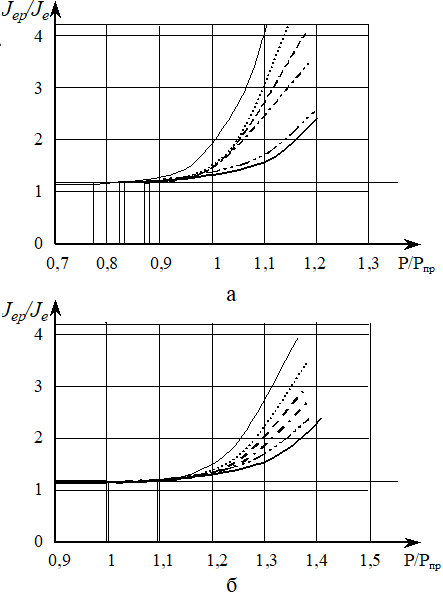
\includegraphics[width=\textwidth]{assets/1148}
		\caption*{Рис. 2 - Графики зависимости $\frac{J_{\text{ep}}}{J_{e}}$ от приложенной нагрузки в образце с центральной трещиной:}
    \end{subfigure}
    \hfill
    \begin{subfigure}[b]{0.45\textwidth}
        \centering
        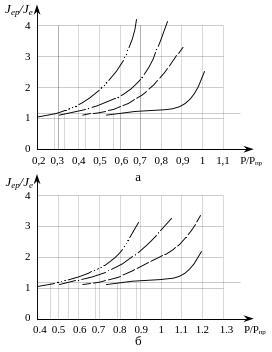
\includegraphics[width=\textwidth]{assets/1150}
		\caption*{Рис. 3 - Графики зависимости $\frac{J_{\text{ep}}}{J_{e}}$ от приложенной нагрузки в образце с краевой трещиной:}
		\caption*{а -- плоское напряженное состояние; б -- плоская деформация}
    \end{subfigure}
\end{figure}

\begin{multicols}{2}
Сказанное выше позволяет перейти к определению аналитических
зависимостей $J$-интеграла в функции
приложенного напряжения, геометрии элемента конструкции с трещиной и
свойств материала. В ряде работ {[}7, 8{]} предложены такие зависимости
в виде:
\end{multicols}

\begin{equation}
J = \alpha \cdot \sigma_{T} \cdot \varepsilon_{T} \cdot \frac{l}{2} \left( 1 - \frac{l}{b} \right) \cdot g_{1} \left( \frac{l}{b}, n \right) \left[ \frac{\sigma \cdot b}{\sigma_{T} \left( b - l \right)} \right]^{n},
\end{equation}

\begin{multicols}{2}
где g\textsubscript{1} - функция отношения длины трещины \emph{l} к
ширине пластины \emph{b} и показателя упрочнения материала n. При этом
предполагается, что материал упрочняется по степенному закону:

\begin{equation}
\frac{\varepsilon}{\varepsilon_{T}} = \alpha \cdot \left( \frac{\sigma}{\sigma_{T}} \right)^{n},
\end{equation}

где α - константа материала, $\varepsilon_{T} = \frac{\sigma_{T}}{E}$ функция
$g_{1} \left( \frac{l}{b}, n \right)$ приводится в табулированном виде
{[}8{]}.

Анализ выражения (1) позволяет заключить, что параметр
$J' = \frac{J}{\alpha \sigma_{T} \varepsilon_{T}}$ зависит только от относительной
длины трещины, приложенной нагрузки и показателя упрочнения \emph{n}.
Так в работе {[}8{]} приведены табулированные значения функции
$g \left( \frac{l}{b}, n \right)$ для образцов с центральной трещиной
для случая плоской деформации. Установить подобное выражение для других
расчетных случаев, характерных для сварных соединений с
непроплавлениями, можно на основе МКЭ и численного эксперимента.

Сказанное выше, распространим на материалы, упрочняющиеся по билинейному
закону. В этом случае, из рассмотрения можно исключить параметр
\emph{n=1.} На основе численного эксперимента было установлено, что
параметр $\frac{J_{p} E_{T}}{\sigma_{T}^{2}}$ не зависит от материала при
развитых пластических деформациях, когда напряжения в нетто-сечении
образца $\sigma_{H} > \sigma_{T}$. Здесь
$J_{p}$-пластический
$J$-интеграл, определяемый как

\begin{equation}
J_{p} = J_{\text{ep}} - J_{e}
\end{equation}

где- упругий
$J_{e}$-интеграл;
$J$-упругопластический
$J_{ep}$-интеграл.

С учетом сказанного можно записать
\end{multicols}

\begin{equation}
J_{\text{ep}} = J_{e} + J_{p} = \frac{K_{I}^{2}}{E'} + \frac{\sigma_{T}^{2} l \left(1 - \frac{l}{b}\right)}{E_{T}} f_{1} \left( \frac{l}{b}, \frac{P}{p_{\text{пр}}} \right)
\end{equation}

\begin{multicols}{2}
где $E'=E$ в случае плоско напряженного
состояния; $E=\frac{E}{1-v^{2}}$в случае плоской
деформации; $f_{1} \left( \frac{l}{b}, \frac{P}{p_{\text{пр}}} \right)$- некоторая функция,
зависящая от относительной длины трещины и уровня приложенной нагрузки.

В выражении (4) величина

\begin{equation*}
\frac{P}{P_{\text{пр}}} = \frac{\sigma b}{\sigma_{T} \left( b - l \right)}.
\end{equation*}

Используя уравнения для $K_{I}${[}9{]},
записанные в общем виде, выражение (4) можно представить в виде
\end{multicols}

\begin{equation}
J_{\text{ep}} = \frac{\sigma^{2} l}{E'} f_{0} \left( \frac{l}{b} \right) + \frac{\sigma_{T}^{2} l \left(1 - \frac{l}{b}\right)}{E_{T}} f_{1} \left( \frac{l}{b}, \frac{P}{P_{\text{пр}}} \right)
\end{equation}

\begin{multicols}{2}
Появление сомножителя ($1-\frac{l}{b}$) связано с
необходимостью удовлетворения выражений (4) и (5) граничным условиям
задачи.

На основе численного эксперимента получены табулированные значения для
функции $f_{1} \left( \frac{l}{b}, \frac{P}{P_{\text{пр}}} \right)$. На рисунках 4 и 5
представлены графические зависимости параметра
$\frac{J_{p} E_{T}}{\sigma_{T}^{2}}$ от длины трещины и приложенной
нагрузки.

На рисунке 6 приведены результаты расчета на основе табулированных
данных для $J$- интеграла (ПНС) в
образце с центральной трещиной зависимости разрушающих напряжений
$\sigma_{c}$ от относительной длины трещины
$\frac{l}{b}$. Расчетные значения хорошо
согласуются с экспериментальными {[}7{]} и уменьшаются с увеличением
длины трещины. Рассматривалась пластина из нержавеющей стали 1X18H9T
($\sigma_{T} = 340 \text{МПа};$ $E = 2 \cdot 10^{5} \text{МПа};$ $J_{c} = 475 \frac{\text{H}}{\text{мм}}$).
Увеличение ширины пластины также приводит к снижению разрушающих
напряжений, причем для пластин с центральной трещиной шириной
$b \geq 300 \text{мм}$ напряжения σ\textsubscript{С}
оказались меньше предела текучести материала
$\left( \frac{l}{b} \geq 0.1 \right)$. В пластине с краевой трещиной такая
ситуация наблюдается уже в пластинах шириной
$b > 100 \text{мм}\ \left( \frac{l}{b} < 0.1 \right)$.
\end{multicols}

\begin{figure}[H]
    \centering
    \begin{subfigure}[b]{0.45\textwidth}
        \centering
        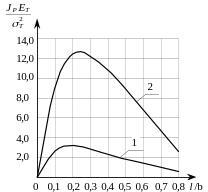
\includegraphics[width=\textwidth]{assets/1188}
		\caption*{Рисунок 4 - Зависимость параметра $\frac{J_{p} E_{T}}{\sigma_{T}^{2}}$ для образца с центральной трещиной (100x200 мм):}
		\caption*{1 -- плоская деформация; 2 --плоское напряженное состояние; \emph{P/P\textsubscript{пр}}=1,4}
    \end{subfigure}
    \hfill
    \begin{subfigure}[b]{0.45\textwidth}
        \centering
        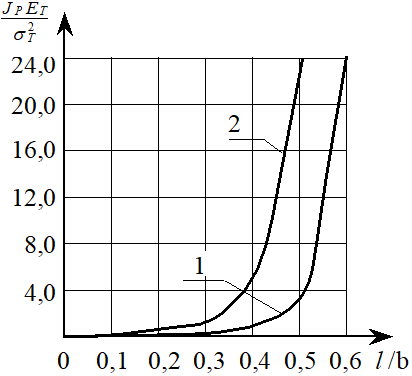
\includegraphics[width=\textwidth]{assets/1190}
		\caption*{Рис. 5 - Зависимость параметра $\frac{J_{p} E_{T}}{\sigma_{T}^{2}}$  для образца с краевой трещиной (100x200 мм):}
		\caption*{1 -- плоская деформация; 2 --плоское напряженное состояние; P/P\textsubscript{пр}=1,4}
    \end{subfigure}
\end{figure}

Можно заключить, что для исследуемой стали расчет по предложенной
формуле дает удовлетворительную погрешность (≈5\%).

\begin{figure}[H]
	\centering
	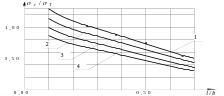
\includegraphics[width=0.45\textwidth]{assets/1192}
	\caption*{Рис. 6 -Зависимость параметра $\frac{\sigma}{\sigma_{0}}$ от относительной длины трещины $\frac{l}{b}$}
	\caption*{1 -- b=70 мм; 2 -- b=150 мм; 3 -- b=300 мм; 4 -- b=600 мм; • - экспериментальные данные} \emph{{[}7{]}}
\end{figure}

\begin{multicols}{2}
{\bfseries Результаты и обсуждения.} Для высокопластичных материалов с
трещинами и вязким характером разрушения, если даже момент страгивания
установлен критерием $J\leq J_{c}$, необходимо
решить задачу распространении трещины, так как характер роста трещины
(устойчивое или неустойчивое) может существенно влиять на
работоспособность и ресурс конструкции. В качестве характеристики
сопротивления материала росту трещины используют
$J_{R}$-кривые {[}10{]}, определяемые
экспериментально. Эти кривые связывают значения
$J$-интеграла с приращением длины
трещины $\Delta l$. Переход к неустойчивому
распространению трещины будет иметь место, если в точке касания
$J$ и
$J_{R}$-кривой выполняются условия

\begin{equation}
J(\sigma, l) = J_{R}(\Delta l)\ \text{и}\ \frac{dJ}{dl} \geq \frac{dJ_{R}}{dl}
\end{equation}

Расчет $J$-кривой (рисунок 7) для стальной пластины с центральной
трещиной проводили по данным {[}9{]} для пластины с центральной
трещиной. $J_{R}$-кривая построена по
данным, полученным с помощью метода делительных сеток {[}7{]}.
\end{multicols}

\begin{figure}[H]
	\centering
	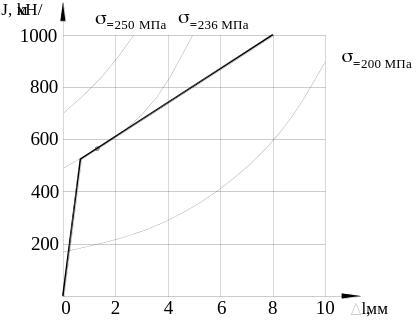
\includegraphics[width=0.45\textwidth]{assets/1204}
	\caption*{Рис. 7 - $J$ и $J_{R}$ - кривые для образца с центральной трещиной для стали 1Х18H9T ($b=70$мм; $\frac{l}{b}=0.5$)}
\end{figure}

\begin{multicols}{2}
Из сопоставления приведенных J и J\textsubscript{R}-кривых (рисунок 7)
следует, что неустойчивое распространение трещины в пластине заданных
размеров в соответствии с условием (6) будет иметь место лишь при
заданной нагрузке. Переход к неустойчивому распространению трещины
произойдет при напряжении σ=236МПа после увеличения трещины на
$\Delta l = 1.3 \text{мм}$ (для сравнения
$\sigma = 223 \text{МПа}, \quad \Delta l = 1.3 \text{мм}$) {[}7{]}.

Представленные данные дают хорошее совпадение с исследованиями других
авторов и в отличие от них являются универсальными для рассматриваемых
классов сталей и законов упрочнения материалов.

Таким образом, зная вязкость разрушения
$J_{IC}$, свойства материала, геометрию
элементов конструкции и ее НДС, можно определить предельную нагрузку,
при которой трещина начнет распространяться.

На основе предложенного в работе подхода {[}9{]} рассмотрим влияние
остаточных сварочных напряжений на величину
$J$-интеграла. В данном случае решается
задача расчета $J$-интеграла в образце
с центральной трещиной при совместном действии внешней нагрузки
$\frac{P}{P_{\text{пр}}}$ и нагрузки на берегах трещины,
эквивалентной действию остаточных напряжений. Рассматривалась пластина
размерами 100x200 мм из Ст3 со следующими характеристиками:
$\sigma_{T} = 250 \text{ МПа};\ E_{T} = 7350 \text{ МПа};\ E = 2 \cdot 10^{5} \text{ МПа}$. В качестве варьируемых параметров
использовались: $\frac{l}{b}$- относительная длина
трещины; $\frac{\sigma_{H}}{\sigma_{T}} = \frac{P}{P_{\text{пр}}}$-приложенная относительная
внешняя нагрузка; $\frac{\sigma_{r}}{\sigma_{T}}$- отношение
нерелаксированных остаточных напряжений к пределу текучести материала. В
результате численного эксперимента оценивались значения функции

\begin{equation}
\psi \left( \frac{\sigma_{H}}{\sigma_{T}}, \frac{\sigma_{r}}{\sigma_{T}}, \frac{l}{b} \right) = \frac{J_{\Sigma}}{J}
\end{equation}

где $J$-энергетический
$J$-интеграл от внешней нагрузки;
$J_{\Sigma}$-энергетический
$J$-интеграл от внешней нагрузки и
нерелаксированных остаточных напряжений.

Предыдущие исследования позволяют принять с некоторой долей приближения,
что функция $\psi \left( \frac{\sigma_{H}}{\sigma_{T}}, \frac{\sigma_{r}}{\sigma_{T}}, \frac{l}{b} \right)$ не зависит от материала
образца. Были приняты следующие диапазоны изменения факторов:
$\frac{l}{b} = \frac{0.1}{0.5};\ \frac{\sigma_{H}}{\sigma_{T}} = \frac{0.22}{1.11};\ \frac{\sigma_{r}}{\sigma_{T}} = \frac{0}{1.0}$
 При этом учитывалось допустимое
сочетание остаточных и приложенных напряжений.

На рисунках 8 и 9 представлены некоторые результаты численного
моделирования. Влияние остаточных напряжений на величину функции
$\psi$ усиливается с ростом длины трещины
и увеличением внешней нагрузки (см. рис.8,
$\sigma_{r}=50$МПа и
$\sigma_{r}=100$МПа). При больших значениях
приложенных напряжений (рис.9) растягивающие остаточные напряжения
релаксируют и почти не оказывают влияния на величину
$J$-интеграла. С понижением
$\sigma$ влияние остаточных напряжений
становится более заметно. Так, если вязкость разрушения
$J_{c} = 240 \frac{\text{H}}{\text{мм}}$ то прочность соединения
уменьшается на 19\% $\left( \frac{\text{OA}_{1}}{\text{OA}_{2}} \approx 1.19 \right)$ за счет
действия нерелаксированных остаточных напряжений. Приведенные данные
свидетельствуют о существенном влиянии остаточных напряжений на
трещиностойкость элементов металлоконструкций, что согласуется с данными
эксперимента {[}9{]}.
\end{multicols}

\begin{figure}[H]
	\centering
	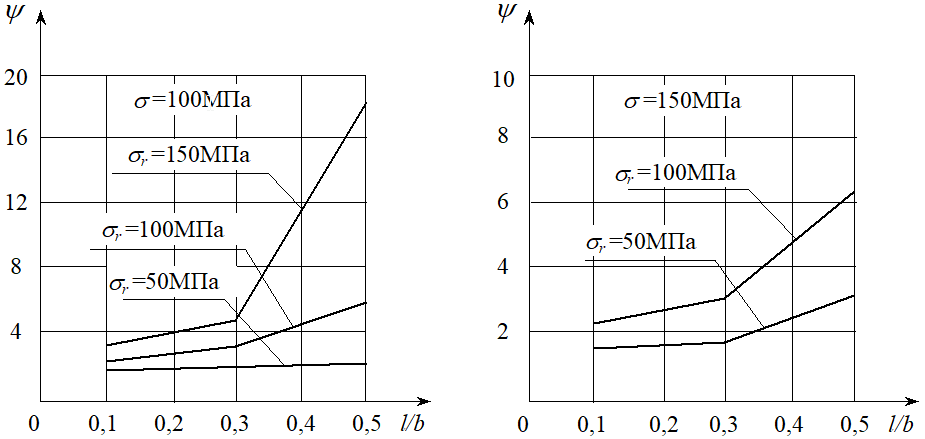
\includegraphics[width=0.8\textwidth]{assets/1237}
	\caption*{Рис. 8 - Зависимость функции $\psi$ от длины трещины, остаточных $\sigma_{r}$ и внешних $\sigma$ напряжений}
\end{figure}

\begin{multicols}{2}
Значение функции $\psi$ приведено в работе
{[}9{]} в табулированном виде. На основе описанного подхода можно
получить подобные функции и для других типов сварных соединений.

Таким образом, зная уровень нерелаксированных остаточных напряжений,
размер дефекта и используя табулированную функцию
$\psi$, можно оценить величину
$J$-интеграла в виде

\begin{equation}
J_{\Sigma} = J \psi \left( \frac{l}{b}, \frac{\sigma_{H}}{\sigma_{T}}, \frac{\sigma_{r}}{\sigma_{T}} \right)
\end{equation}
\end{multicols}

\begin{figure}[H]
	\centering
	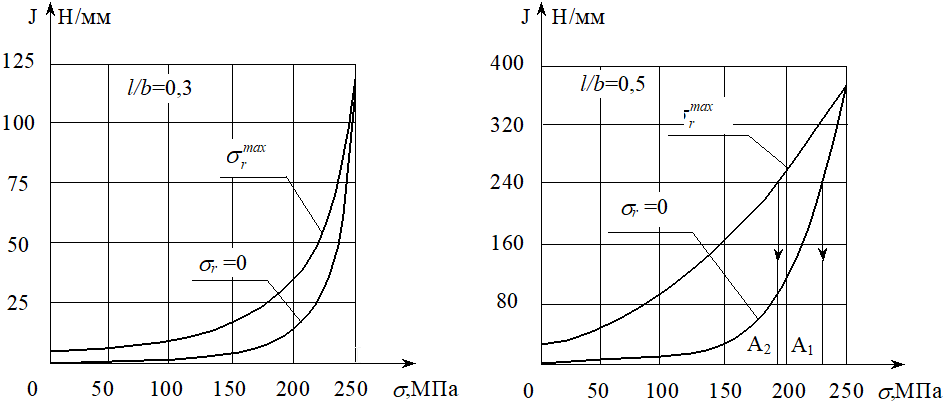
\includegraphics[width=0.8\textwidth]{assets/1245}
	\caption*{Рис. 9 - Влияние нерелаксированных остаточных напряжений на величину \emph{J}-интеграла}
\end{figure}

Здесь значение $J$-интеграла
от действия внешней нагрузки и длины трещины определяем на основе
табулированных данных {[}9{]}.

{\bfseries Выводы.} В данной работе с помощью полученных регрессионых
зависимостей решены следующие задачи.

Определены границы применяемости линейной механики разрушения для
краевых и центральных трещин в типичных образцах.

Установлены зависимости разрушающих напряжений
$\sigma_{c}$ от относительной длины трещины
$\frac{l}{b}$ в образцах с центральной и краевой
трещинами на основе $J$-интеграла.

Оценено влияние остаточных напряжений на величину \emph{J}-интеграла в
типовых образцах.

Таким образом, регрессионные зависимости для определения
\emph{J}-интеграла обладают достаточной надежностью и могут
использоваться в практике прогнозирования остаточного ресурса сварных
металлоконструкций.

\begin{center}
{\bfseries Литература}
\end{center}

\begin{noparindent}
1. Richard, H., Sander, M., Fulland, M. and Kullmer, G. Development of
fatigue crack growth in real structures // Engineering Fracture
Mechanics. - 2008. -- Vol. 75. - P. 331-340. DOI
10.1016/j.engfracmech.2007.01.017

2. Ghosh A., Barman N., Chattopadhyay H., Hloch S. A study of thermal
behaviour during submerged arc welding.// J Mech Eng.- 2013.- Vol.
59(5)- P. 333-338. DOI 10.5545/sv-jme.2012.775

3. Zhu M.-L., Xuan F.-Z. and Tu S.-T. Effect of load ratio on fatigue
crack growth in the near-threshold regime: A literature review, and a
combined crack closure and driving force approach//Engineering Fracture
Mechanics.- 2015.- Vol. 141.- P. 57-77. DOI
10.1016/j.engfracmech.2015.05.005

4. Besel, M. and Breitbarth, E. Advanced analysis of crack tip plastic
zone under cyclic loading// International Journal of Fatigue. -2016. -
Vol. 93(1).-P. 92-108. DOI 10.1016/j.ijfatigue.2016.08.013

5. Lopez-Crespo, P., Shterenlikht, A., Patterson, E. A., Yates, J. R.
and Withers, P. J. The stress intensity of mixed mode cracks determined
by digital image correlation // Journal of strain analsysis for
engineering design.-2008. -Vol. 43. - P. 769-780. DOI
10.1243/03093247JSA419

6. Нұрғожин М.Р., Даненова Г.Т., Сайлауқызы Ж.Қалдық дәнекерлеу
кернеулеріне және деформацияға механикалық әсердің әсерін компьютерлік
модельдеу // Университ Еңбектері ҚарМТУ.-2020-№ 3(80).-С.19-24. DOI
10.25209/1609- 1825\_2020\_3\_19

7. Nurguzhin M., Danenova G., Akhmetzhanov T. Computer modeling of the
stress-strain state of welded

construction// in AIP Conf Proc. -
Prospects of fundamental sciences development (PFSD-2017).- Tomsk.-
2017.- V.1899 (1). DOI 10.1063/1.5009879

8. Traidia A., Roger F. Numerical and experimental study of arc and weld
pool behavior for pulsed current GTA welding.// Int J Heat Mass Tran.-
2011.- Vol. 54 (9-10).- P.2163-2179. DOI
10.1016/j.ijheatmasstransfer.2010.12.005

9. Нургужин М.Р., Даненова Г.Т. Основы расчета характеристик живучести
сварных металлоконструкций: монография. - Караганда. Изд-во КарТУ.-
2021.- 133 с.

10. Нургужин М.Р., Даненова Г.Т. Моделирование тепловых процессов в
сварных соединениях: монография. -Караганда: Изд-во НАО «КарТУ имени
Абылкаса Сагинова».- 2023.- 83 с.
\end{noparindent}

\begin{center}
{\bfseries References}
\end{center}

\begin{noparindent}
1. Richard, H., Sander, M., Fulland, M. and Kullmer, G. Development of
fatigue crack growth in real structures // Engineering Fracture
Mechanics. - 2008. -- Vol. 75. - P. 331-340. DOI
10.1016/j.engfracmech.2007.01.017

2. Ghosh A., Barman N., Chattopadhyay H., Hloch S. A study of thermal
behaviour during submerged arc welding.// J Mech Eng.- 2013.- Vol.
59(5)- P. 333-338. DOI 10.5545/sv-jme.2012.775

3. Zhu M.-L., Xuan F.-Z. and Tu S.-T. Effect of load ratio on fatigue
crack growth in the near-threshold regime: A literature review, and a
combined crack closure and driving force approach//Engineering Fracture
Mechanics.- 2015.- Vol. 141.- P. 57-77. DOI
10.1016/j.engfracmech.2015.05.005

4. Besel, M. and Breitbarth, E. Advanced analysis of crack tip plastic
zone under cyclic loading// International Journal of Fatigue. -2016. -
Vol. 93(1).-P. 92-108. DOI 10.1016/j.ijfatigue.2016.08.013

5. Lopez-Crespo, P., Shterenlikht, A., Patterson, E. A., Yates, J. R.
and Withers, P. J. The stress intensity of mixed mode cracks determined
by digital image correlation // Journal of strain analsysis for
engineering design.-2008. -Vol. 43. - P. 769-780. DOI
10.1243/03093247JSA419

6. Nūrğojin M.R., Danenova G.T., SailauqyzyJ.Qaldyq dänekerleu
kerneulerıne jäne deformasiağa mehanikalyq äserdıñ äserın kömpüterlık
modeldeu // Universit Eñbekterı QarMTU.-2020-№ 3(80).-S.19-24. DOI
10.25209/1609- 1825\_2020\_3\_19 {[}in Kazakh{]}

7. Nurguzhin M., Danenova G., Akhmetzhanov T. Computer modeling of the
stress-strain state of welded

construction// in AIP Conf Proc. -
Prospects of fundamental sciences development (PFSD-2017).- Tomsk.-
2017.- V.1899 (1). DOI 10.1063/1.5009879

8. Traidia A., Roger F. Numerical and experimental study of arc and weld
pool behavior for pulsed current GTA welding.// Int J Heat Mass Tran.-
2011.- Vol. 54 (9-10).- P.2163-2179. DOI
10.1016/j.ijheatmasstransfer.2010.12.005

9. Nurguzhin M.R., Danenova G.T. Osnovy rascheta kharakteristik
zhivuchesti svarnykh metallokonstruktsii: monografiya. - Karaganda.
Izd-vo KarTU.- 2021.- 133 s. {[}in Russian{]}

10. Nurguzhin M.R., Danenova G.T. Modelirovanie teplovykh protsessov v
svarnykh soedineniyakh: monografiya. -Karaganda: Izd-vo NAO «KarTU imeni
Abylkasa Saginova».- 2023.- 83 s. {[}in Russian{]}
\end{noparindent}

\emph{{\bfseries Сведения об авторах}}

\begin{noparindent}
Нургужин М.Р. - доктор технических наук, профессор, Акционерное общество
«Национальный центр космических исследований и технологий», Алматы,
Казахстан, e-mail: maratnurg57@mail.ru;

Даненова Г.Т. - кандидат технических наук, доцент, Карагандинский
технический университет имени Абылкаса Сагинова, Караганда, Казахстан,
e-mail: guldan72@mail.ru;

Нургужина А.М. - кандидат технических наук, доцент, Astana IT
университет, Астана, Казахстан, e-mail:
assel.nurguzhina@astanait.edu.kz;

Ахметжанов Т.Б. -кандидат технических наук, доцент, Карагандинский
технический университет имени Абылкаса Сагинова, Караганда, Казахстан,
e-mail: akhmetzhantalgat@gmail.com
\end{noparindent}

\emph{{\bfseries Information about the authors}}

\begin{noparindent}
Nurguzhin M.R. - Doctor of Technical Sciences, Professor, Joint Stock
Company ``National Center of Space Researches and Technologies'',
Almaty, Kazakhstan, e-mail: maratnurg57@mail.ru;

Danenova G.T. - Сandidate of Technical Sciences, Associate Professor,
Karaganda Technical University named by Abylkas Saginov, Karaganda,
Kazakhstan, e-mail: guldan72@mail.ru;

Nurguzhinа А.M. - Сandidate of Technical Sciences, Associate Professor,
Astana IT University, Astana, Kazakhstan, e-mail:
assel.nurguzhina@astanait.edu.kz;

Akhmetzhanov T.B. - Сandidate of Technical Sciences, Associate
Professor, Karaganda Technical University named by Abylkas Saginov,
Karaganda, Kazakhstan, e-mail: akhmetzhantalgat@gmail.com\newpage
\end{noparindent}
